
\begin{frame}{Aplicación para entrenamiento de Spelling (1)}
\begin{block}{Motivación} 
Es necesario una herramienta que apoye a los padres a entrenar a sus hijos para concursos de Spelling
\begin{itemize}
\item El usuario ingresa las palabras
\item La aplicacion muestra el deletro de dicha palabra
\item Mediante el sintetizador de voz, es posible leer toda la palabra o el deletreo de la misma para corregir
\item La lista de palabras se va guardando de manera local, no es necesario volver a escribirla
\item Es posible hacer correcciones a las palabras ingresadas
\end{itemize}
\end{block} 
\end{frame}


\begin{frame}{Aplicación para entrenamiento de Spelling (2)}
%\begin{block}{Pantallas Principales} 
\begin{center}
	\begin{tabular}{cc}
		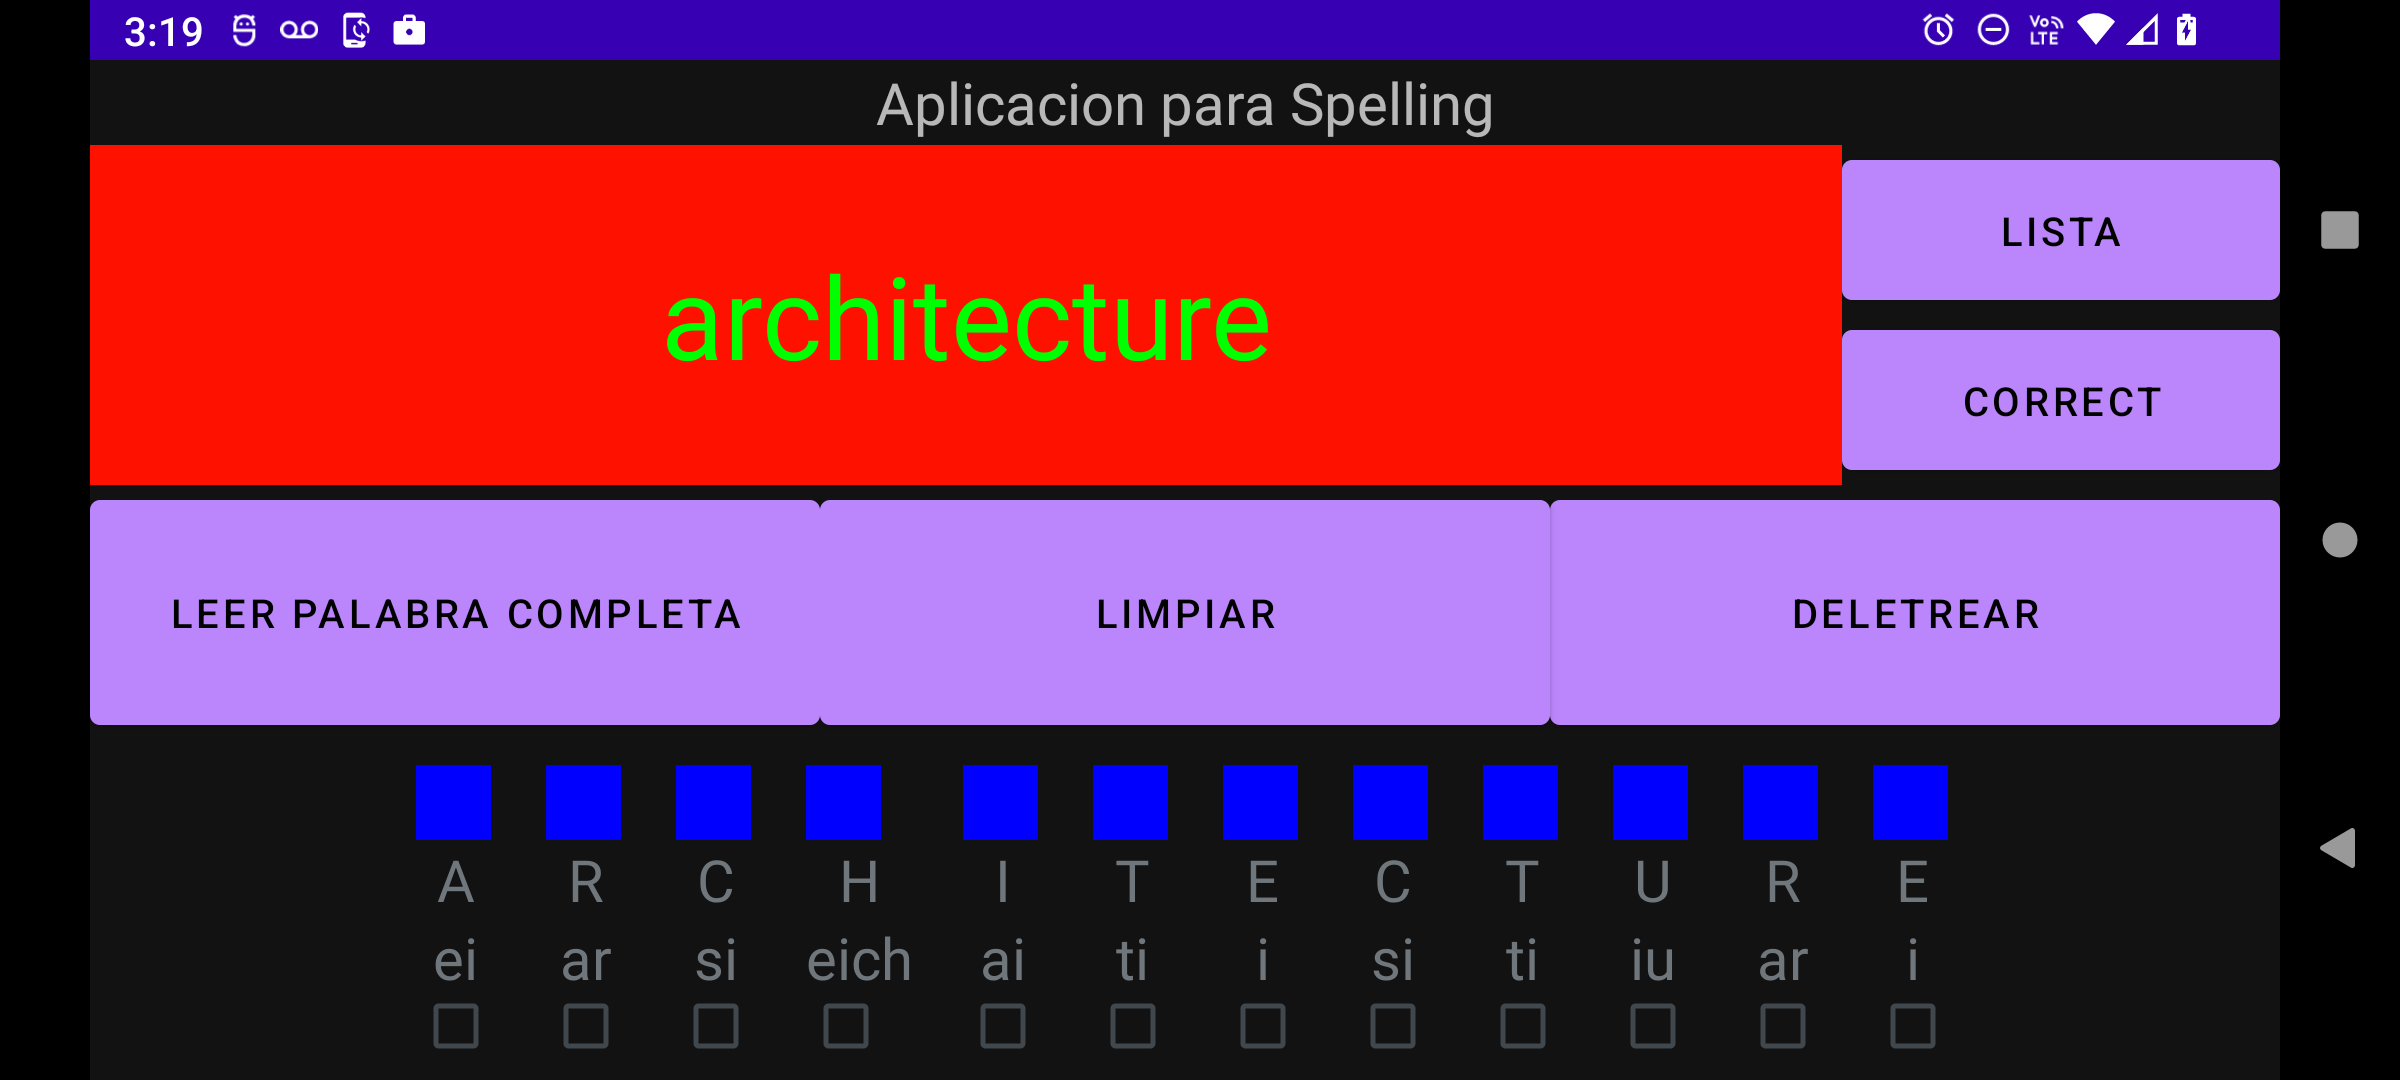
\includegraphics[width=0.46\linewidth]{2022_Spelling/figs/Spelling0.png} &
		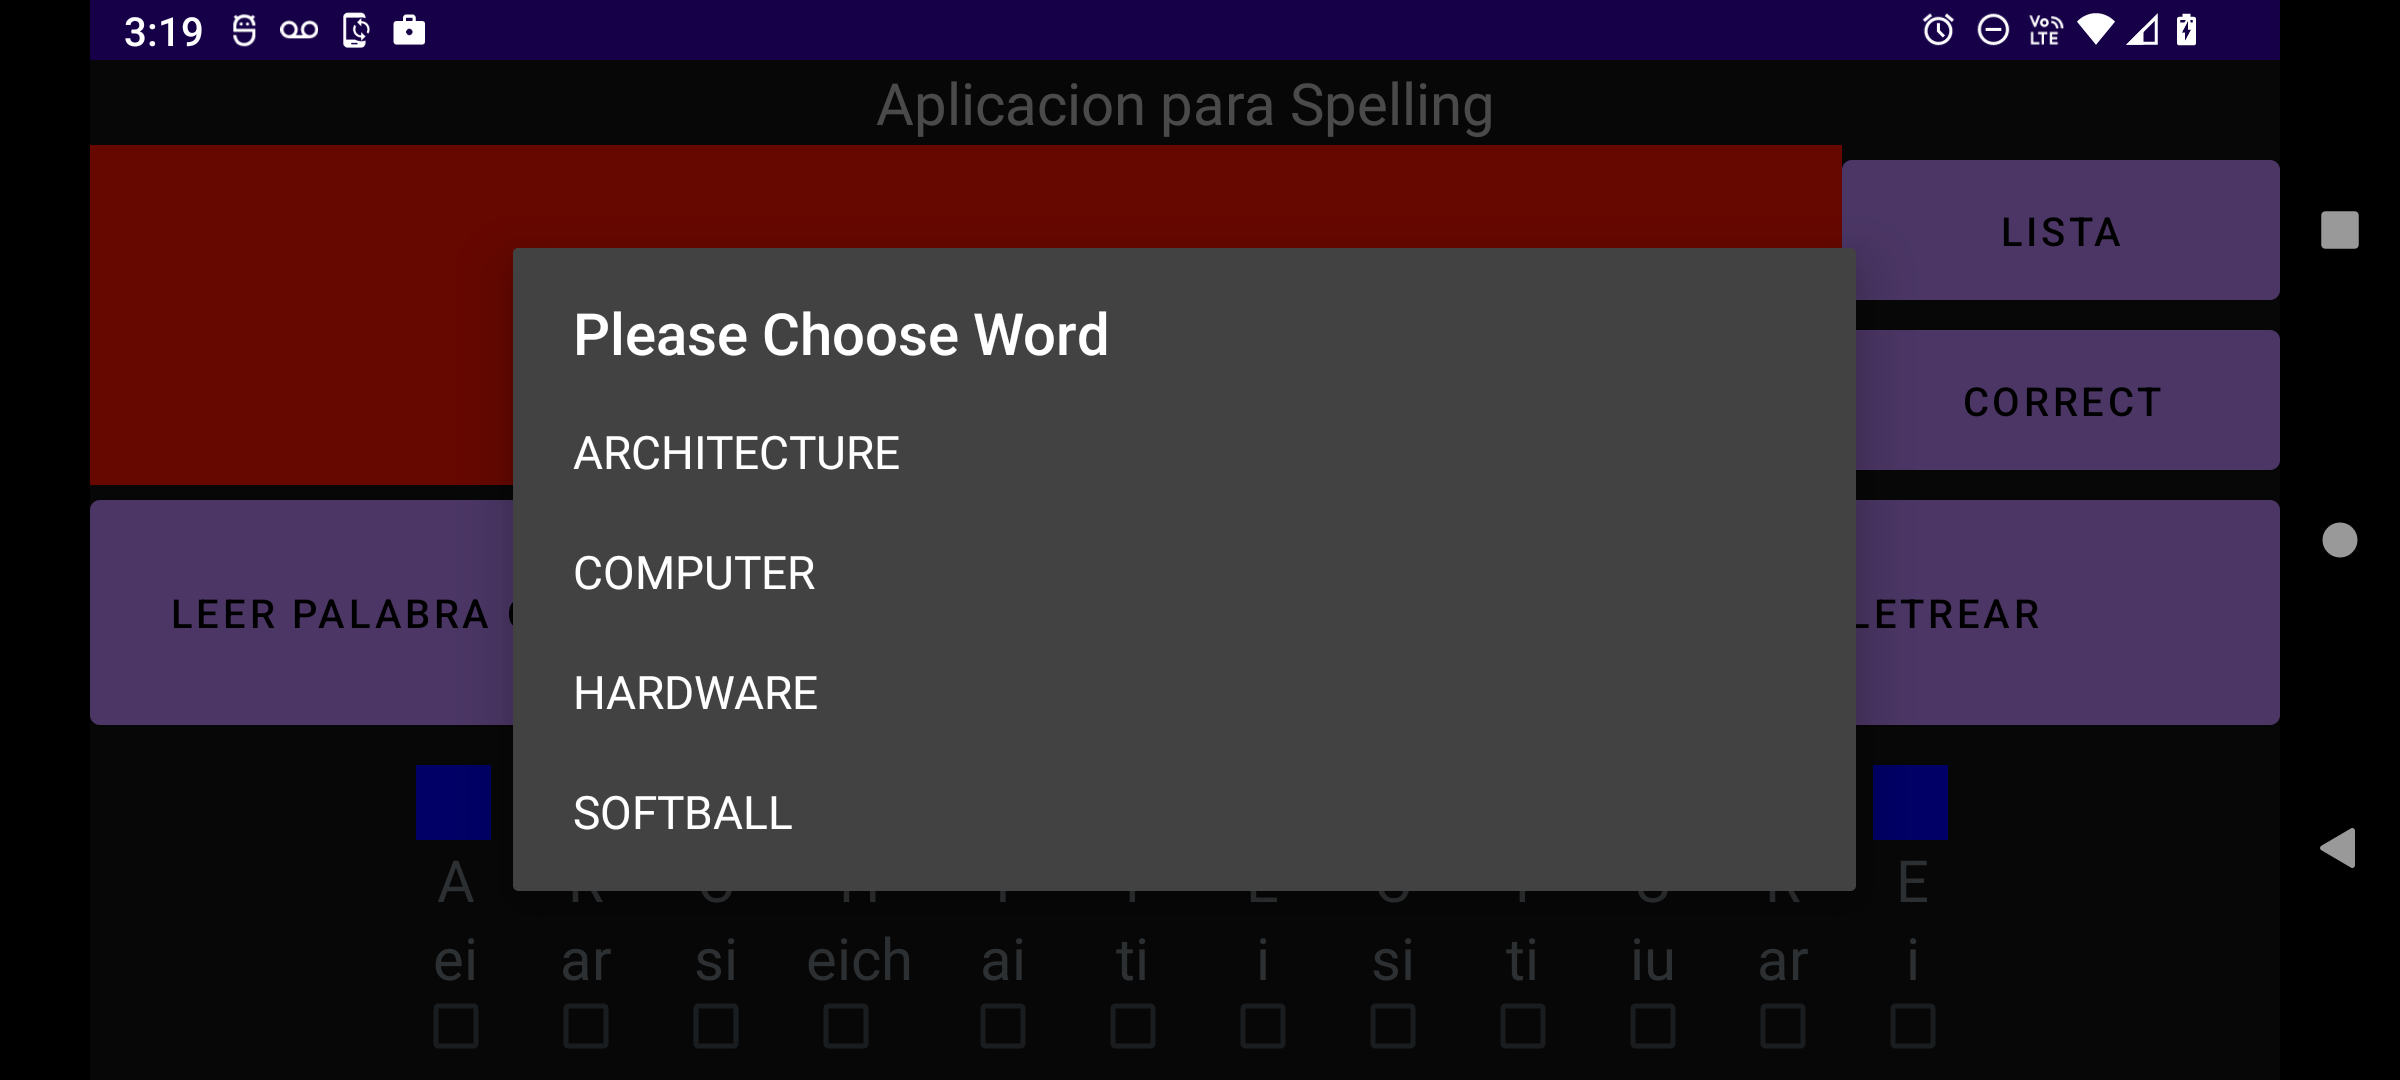
\includegraphics[width=0.46\linewidth]{2022_Spelling/figs/Spelling1.png} \\ 		 		
		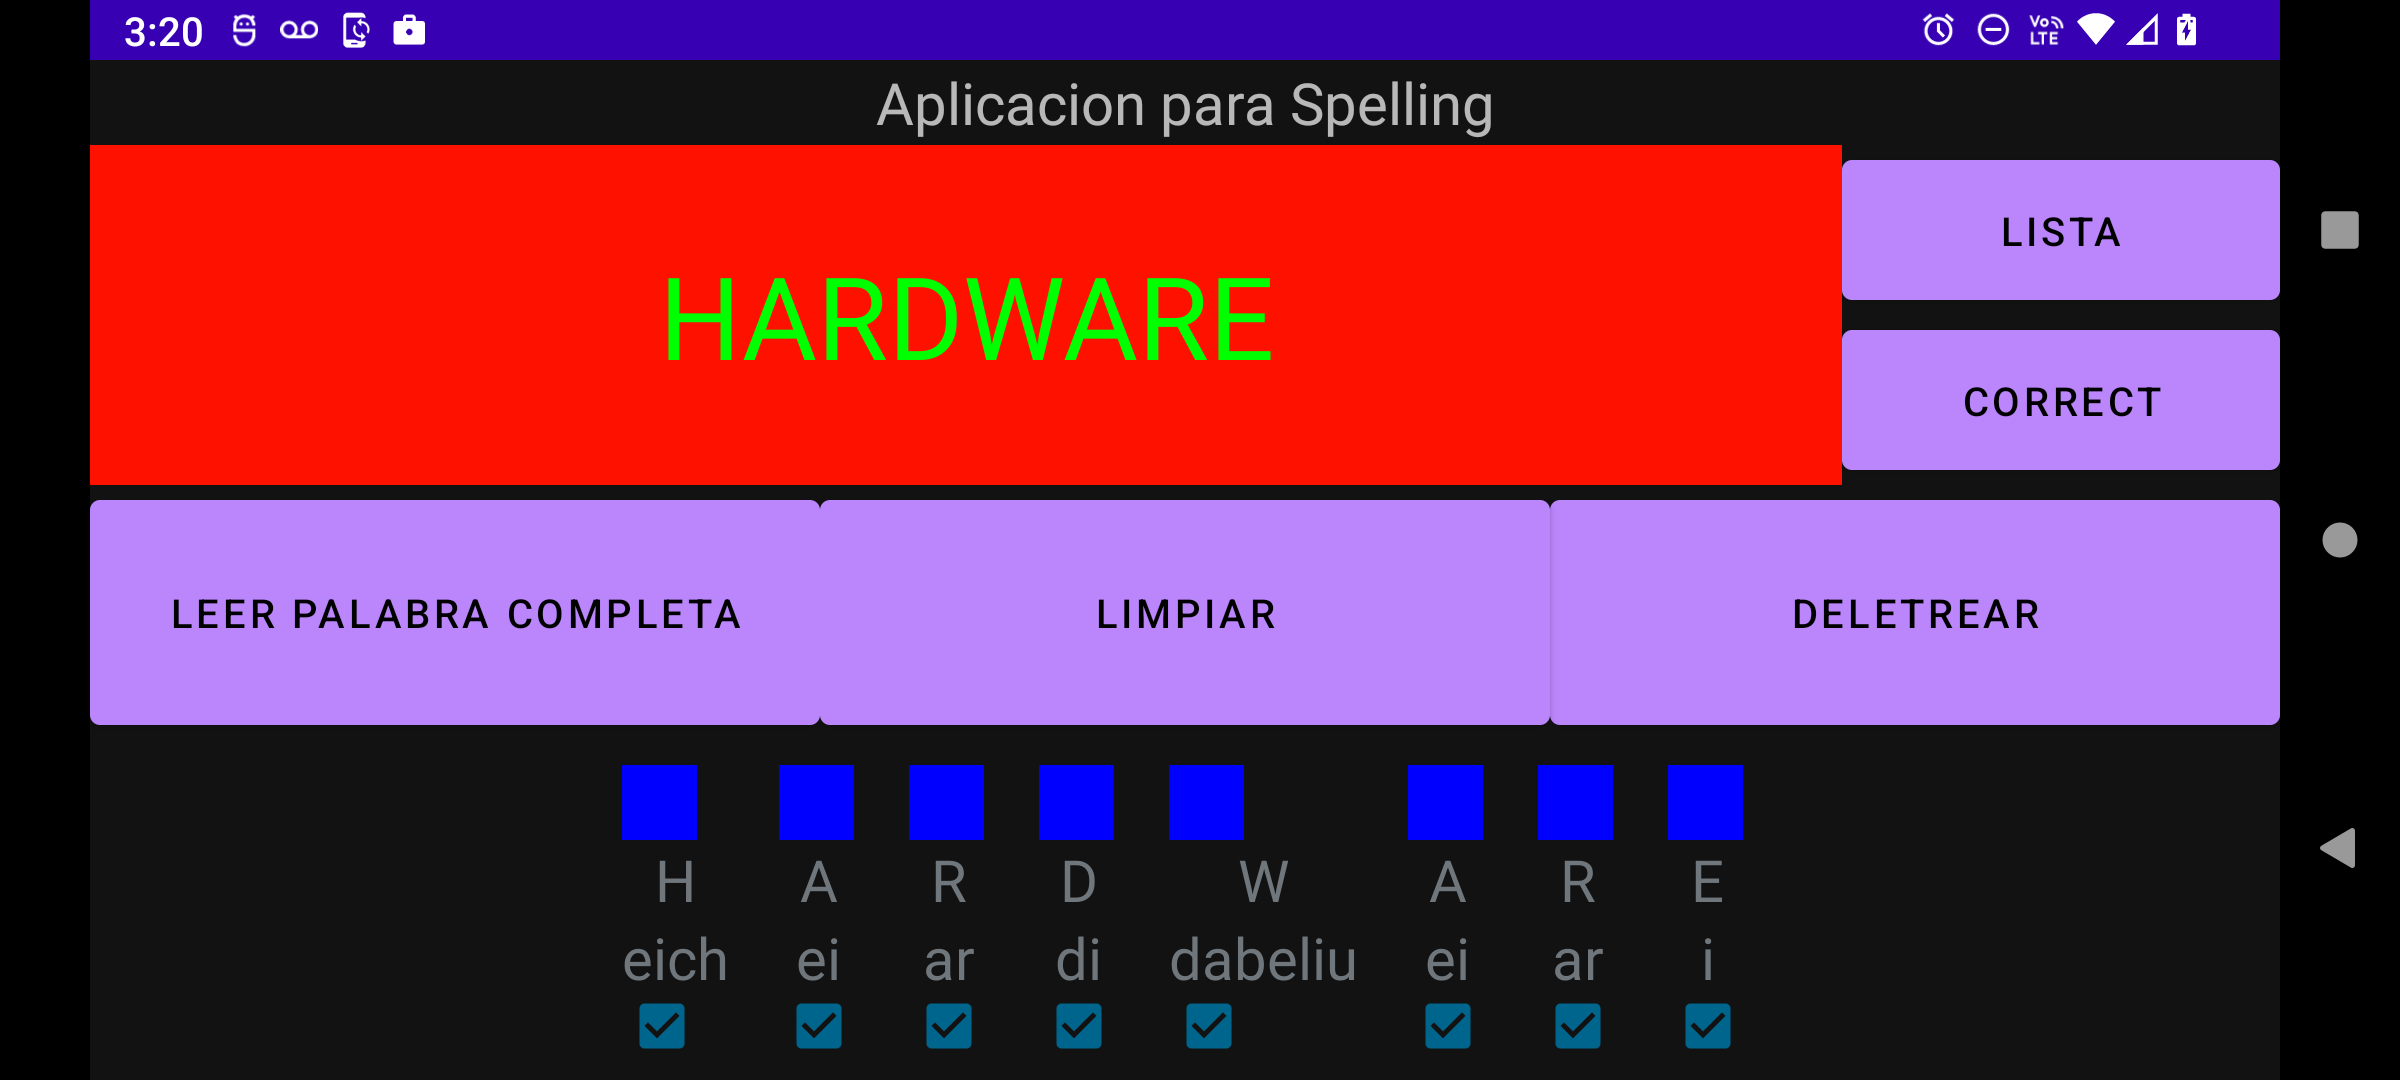
\includegraphics[width=0.46\linewidth]{2022_Spelling/figs/Spelling2.png} & 		
		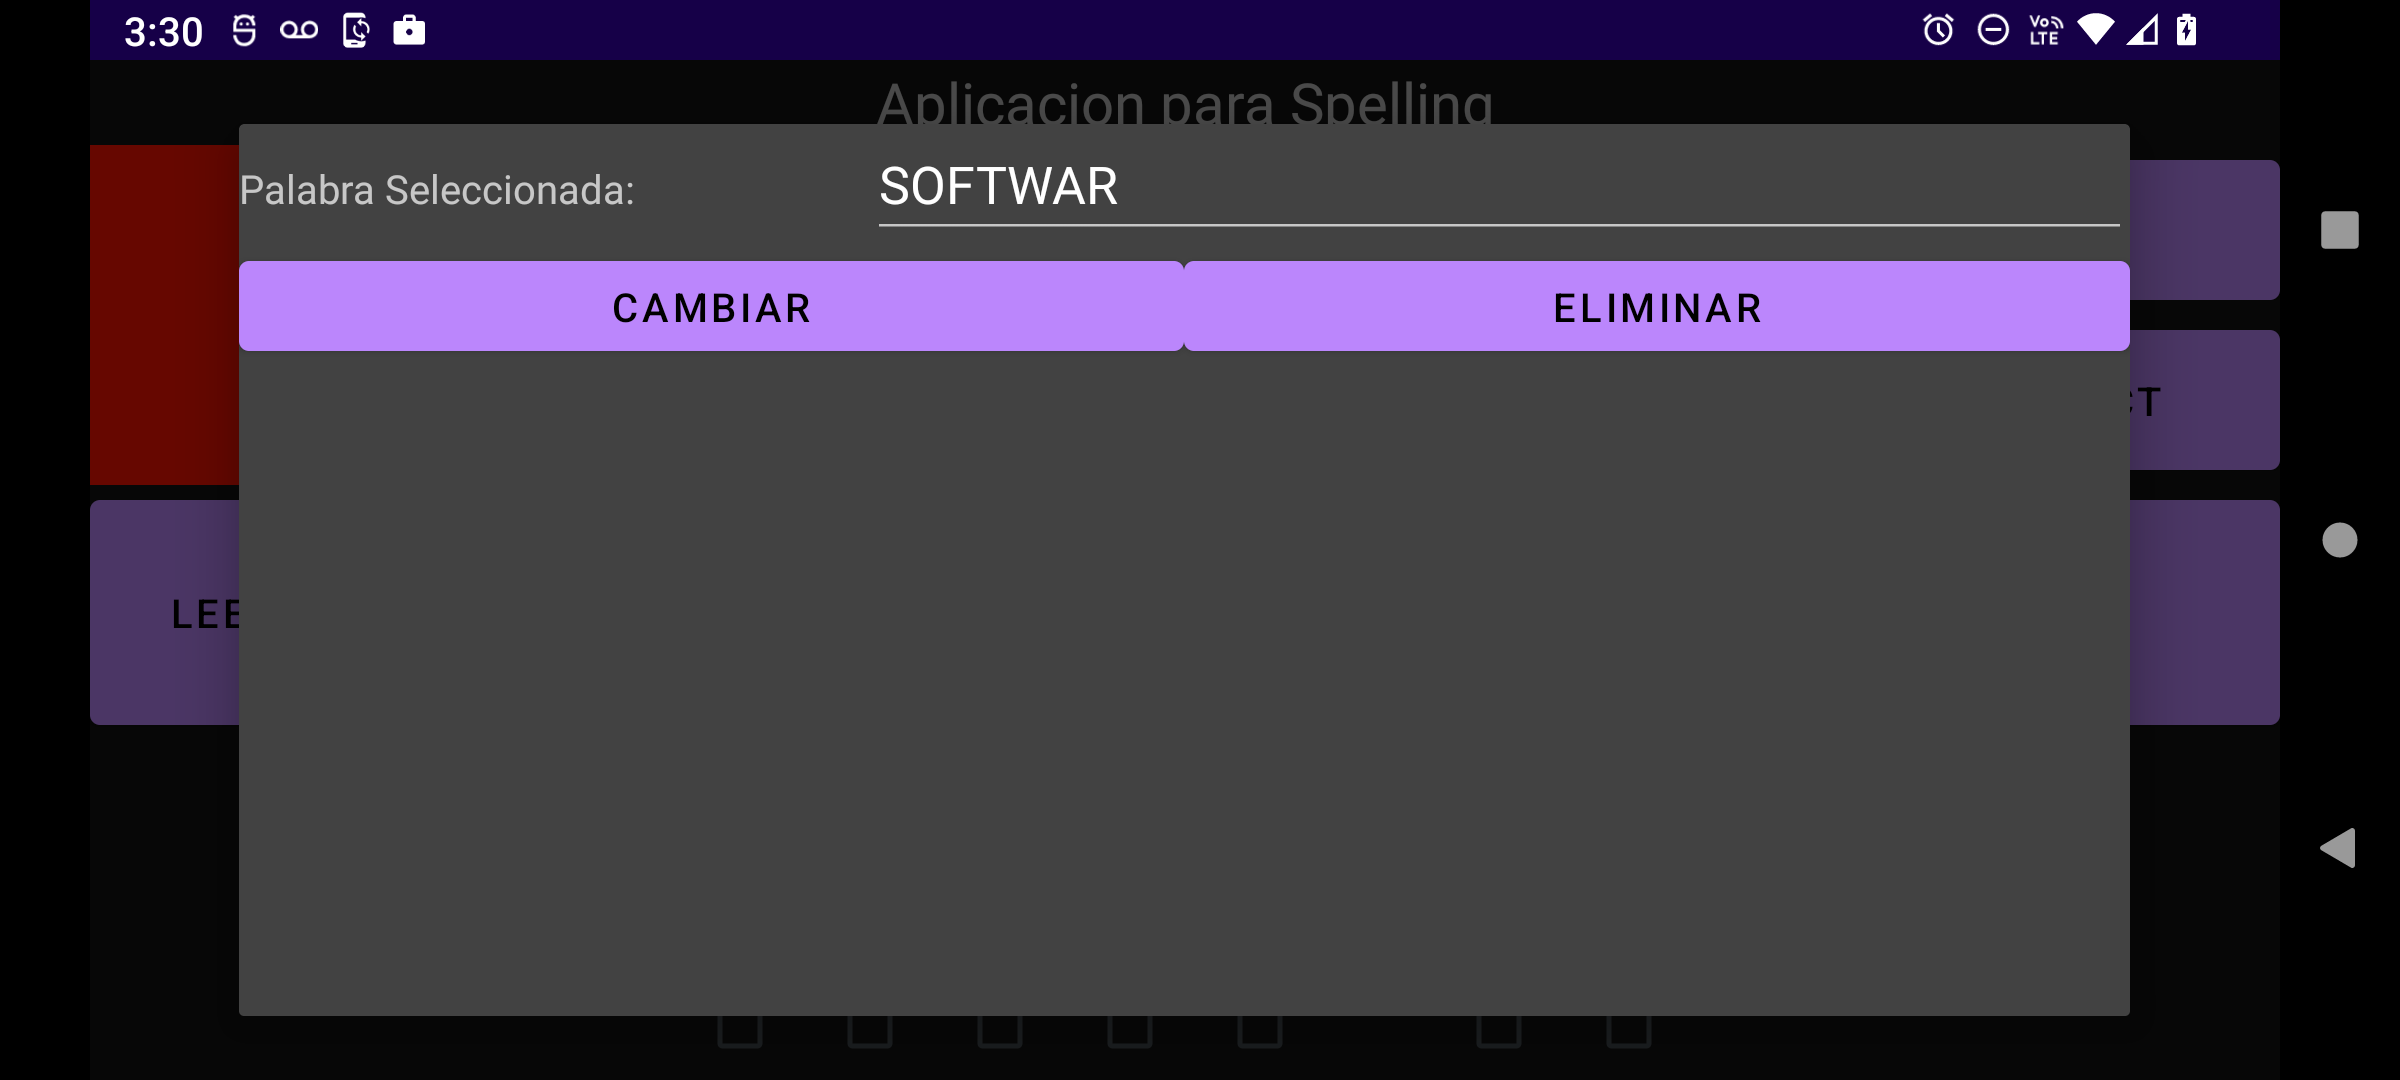
\includegraphics[width=0.46\linewidth]{2022_Spelling/figs/Spelling3.png} \\
	\end{tabular}
\end{center}
\end{frame}

